\subsubsection{Struttura dell'Architettura Transformer}

Il modello Transformer è composto principalmente da due componenti chiave: l'encoder e il decoder. Questi due componenti sono spesso usati insieme in diverse applicazioni di NLP, come la traduzione automatica, la generazione di testo e molte altre.

\subsection{Encoder}
L'encoder trasforma l'input (ad esempio, una sequenza di parole) in un insieme di rappresentazioni chiamate "embeddings" che catturano informazioni semantiche e strutturali. L'encoder è composto da più strati identici, ciascuno dei quali ha due componenti principali:

Multi-Head Self-Attention Layer: Questo è il cuore del modello Transformer. In questa parte, l'input (che è una sequenza di vettori) viene diviso in tre versioni: Query, Key e Value. L'attenzione self-attention calcola l'importanza delle diverse parti dell'input rispetto a ogni altra parte. Ciò consente al modello di catturare relazioni di lungo raggio tra le parole. Vengono eseguiti diversi calcoli di attenzione in parallelo (multi-head) per catturare diverse aspetti delle relazioni tra le parole.

Feedforward Neural Network: Dopo l'operazione di attenzione, l'output viene passato attraverso un'operazione di feedforward in cui ogni vettore di input viene trasformato tramite uno strato completamente connesso.

L'output di ogni strato dell'encoder è l'input per lo strato successivo. La pila di questi strati aiuta a catturare informazioni sempre più astratte e complesse dalle sequenze di input.

\subsection{Decoder}
Il decoder è responsabile di generare l'output a partire dalla rappresentazione creata dall'encoder. Anche il decoder è composto da diversi strati, ma include anche alcune differenze rispetto all'encoder:

Masked Multi-Head Self-Attention Layer: Invece di avere un'attenzione self-attention standard, il decoder utilizza un'attenzione self-attention mascherata. Ciò significa che in ogni posizione, una parola può "guardare" solo le parole che la precedono. Questo impedisce al modello di imbrogliare guardando le parole future durante la generazione.

Multi-Head Encoder-Decoder Attention Layer: Questo strato consente al decoder di concentrarsi sulle parti rilevanti dell'output dell'encoder. Aiuta a catturare le informazioni necessarie dall'input per generare l'output corretto.

Feedforward Neural Network: Simile all'encoder, il decoder ha anche strati di reti neurali feedforward per elaborare ulteriormente l'output.

In entrambi gli encoder e decoder, tra i vari strati, sono spesso utilizzati la normalizzazione batch e i collegamenti residui per facilitare l'allenamento e mitigare i problemi di vanishing gradient.

Nella figura~\ref{fig:transformer} è possibile vedere la struttura dell'architettura Transformer con a sinistra la parte di encoder e a destra la parte di decoder.

Quando si tratta di compiti specifici, come la traduzione automatica, il modello viene addestrato a generare la sequenza di output passo dopo passo, prendendo in considerazione l'output generato in passaggi precedenti. Durante l'allenamento, viene utilizzata una funzione di perdita che misura quanto bene l'output generato si avvicina all'output di riferimento desiderato.

\begin{center}
    \begin{figure}[H]
        \centering
        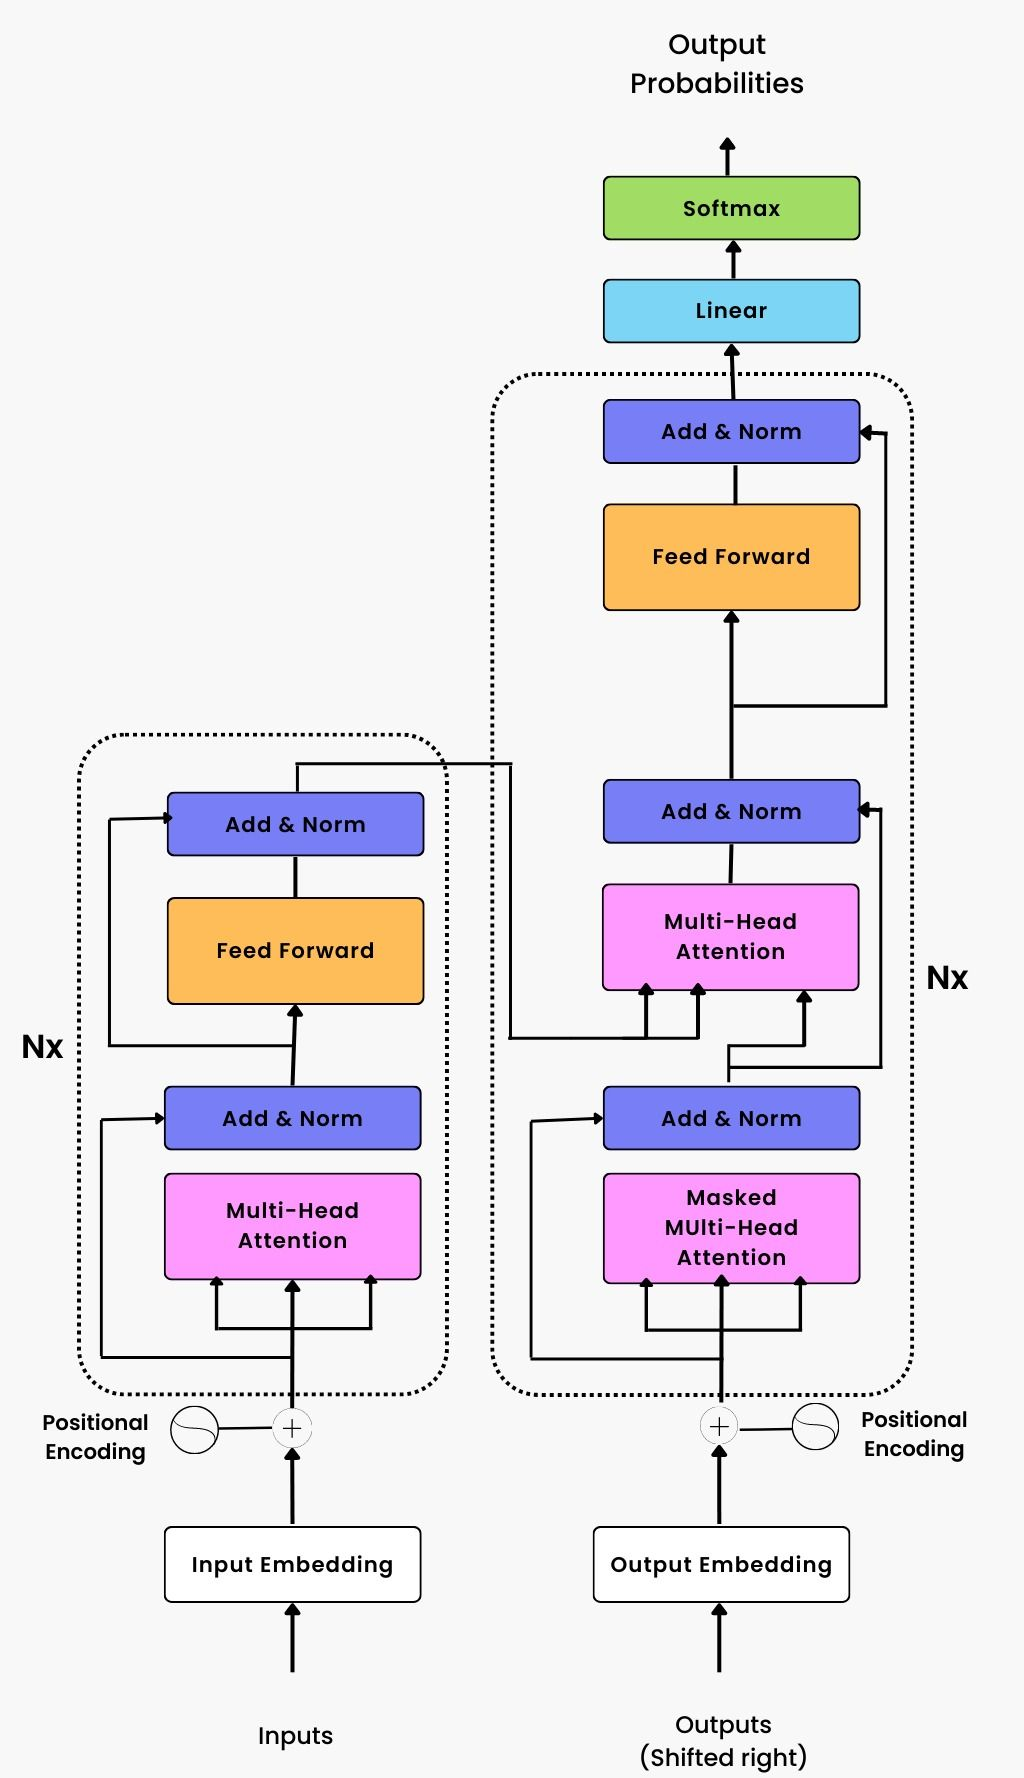
\includegraphics[width=0.5\pdfpagewidth]{images/Transformer.png}
        \caption{La struttura dell'architettura Transformer}
        \label{fig:transformer}
    \end{figure}
    
\end{center}

\subsection{Applicazioni nell'NLP}
I Transformer sono stati applicati con successo a molteplici task di NLP, tra cui traduzione automatica, analisi del sentimento, generazione di testo, risposta alle domande e molto altro. Grazie alla capacità dell'architettura di catturare relazioni complesse, i modelli basati su Transformer hanno raggiunto o superato le prestazioni umane in molti di questi task.

\subsection{Scalabilità e parallelismo}
Una caratteristica distintiva dei Transformer è la loro scalabilità orizzontale. A causa dell'indipendenza dei calcoli di attenzione tra le diverse parole di una sequenza, i Transformer possono eseguire calcoli paralleli su GPU e TPU, accelerando notevolmente l'addestramento e l'inferenza.

\subsection{Limitazioni e sviluppi successivi}
I modelli Transformer hanno rappresentato un passo significativo nell'ambito dell'apprendimento automatico e del trattamento del linguaggio naturale (NLP). Tuttavia, come qualsiasi tecnologia, hanno delle limitazioni e hanno visto alcuni sviluppi successivi. Ecco una panoramica delle limitazioni e degli sviluppi:

Le limitazioni principali riguardano:
\begin{itemize}
    \item Requisiti computazionali elevati: I modelli Transformer richiedono enormi risorse computazionali per l'addestramento e l'inferenza. Questo rende difficile l'accesso a tali modelli per la maggior parte dei ricercatori e delle organizzazioni.
    \item Memoria limitata: Anche se i Transformer possono trattare sequenze lunghe, la loro memoria è comunque limitata. Questo può portare a problemi di prestazioni quando si lavora con testi estremamente lunghi.
    \item Mancanza di comprensione semantica: I modelli Transformer eccellono nel generare testo coerente, ma spesso mancano di una vera comprensione semantica del linguaggio. Possono produrre risposte sbagliate o non coerenti.
    \item Apprendimento basato su grandi quantità di dati: I Transformer richiedono enormi quantità di dati per l'addestramento. Questo può portare a problemi di bias e a una dipendenza da dati di bassa qualità o tendenziosi.
\end{itemize}

Delle possibili soluzioni a queste limitazioni sono rappresentate dai vari ambiti in cui la ricerca si sta muovendo,nonostante i limiti computazionali, i ricercatori continuano a sviluppare modelli Transformer sempre più grandi, come GPT-4 e successivi. Questi modelli tendono a migliorare le prestazioni, ma richiedono hardware di fascia alta.
I ricercatori stanno cercando di rendere i modelli Transformer più efficienti dal punto di vista computazionale, ad esempio utilizzando quantizzazione dei pesi, pruning e altre tecniche di compressione dei modelli.
Sono stati inoltr sviluppati modelli Transformer in grado di gestire più lingue simultaneamente, rendendo il NLP più accessibile a livello globale, il solo GPT-3.5 supporta 12 lingue, comprese quelle con alfabeti non occidentali.
Sono stati sviluppati modelli Transformer specializzati per compiti specifici, come il riconoscimento del linguaggio naturale medico o il trattamento di lingue a bassa risorsa.
C'è inoltre una crescente attenzione al problema del bias nei modelli Transformer e agli sforzi per garantire una maggiore equità nei risultati prodotti da questi modelli.

In sintesi, i modelli Transformer hanno rivoluzionato il campo del NLP, ma presentano ancora alcune sfide importanti. Gli sviluppi futuri si concentreranno sull'efficienza, sull'equità e sulla comprensione semantica più profonda per rendere questi modelli ancora più utili e accessibili.